%Version 3.1 December 2024
% See section 11 of the User Manual for version history
%
%%%%%%%%%%%%%%%%%%%%%%%%%%%%%%%%%%%%%%%%%%%%%%%%%%%%%%%%%%%%%%%%%%%%%%
%%                                                                 %%
%% Please do not use \input{...} to include other tex files.       %%
%% Submit your LaTeX manuscript as one .tex document.              %%
%%                                                                 %%
%% All additional figures and files should be attached             %%
%% separately and not embedded in the \TeX\ document itself.       %%
%%                                                                 %%
%%%%%%%%%%%%%%%%%%%%%%%%%%%%%%%%%%%%%%%%%%%%%%%%%%%%%%%%%%%%%%%%%%%%%

%%\documentclass[referee,sn-basic]{sn-jnl}% referee option is meant for double line spacing

%%=======================================================%%
%% to print line numbers in the margin use lineno option %%
%%=======================================================%%

%%\documentclass[lineno,pdflatex,sn-basic]{sn-jnl}% Basic Springer Nature Reference Style/Chemistry Reference Style

%%=========================================================================================%%
%% the documentclass is set to pdflatex as default. You can delete it if not appropriate.  %%
%%=========================================================================================%%

%%\documentclass[sn-basic]{sn-jnl}% Basic Springer Nature Reference Style/Chemistry Reference Style

%%Note: the following reference styles support Namedate and Numbered referencing. By default the style follows the most common style. To switch between the options you can add or remove Numbered in the optional parenthesis.
%%The option is available for: sn-basic.bst, sn-chicago.bst%

%%\documentclass[pdflatex,sn-nature]{sn-jnl}% Style for submissions to Nature Portfolio journals
%%\documentclass[pdflatex,sn-basic]{sn-jnl}% Basic Springer Nature Reference Style/Chemistry Reference Style
\documentclass[pdflatex,sn-mathphys-num]{sn-jnl}% Math and Physical Sciences Numbered Reference Style
%%\documentclass[pdflatex,sn-mathphys-ay]{sn-jnl}% Math and Physical Sciences Author Year Reference Style
%%\documentclass[pdflatex,sn-aps]{sn-jnl}% American Physical Society (APS) Reference Style
%%\documentclass[pdflatex,sn-vancouver-num]{sn-jnl}% Vancouver Numbered Reference Style
%%\documentclass[pdflatex,sn-vancouver-ay]{sn-jnl}% Vancouver Author Year Reference Style
%%\documentclass[pdflatex,sn-apa]{sn-jnl}% APA Reference Style
%%\documentclass[pdflatex,sn-chicago]{sn-jnl}% Chicago-based Humanities Reference Style

%%%% Standard Packages
%%<additional latex packages if required can be included here>

\usepackage{graphicx}%
\usepackage{multirow}%
\usepackage{amsmath,amssymb,amsfonts}%
\usepackage{amsthm}%
\usepackage{mathrsfs}%
\usepackage[title]{appendix}%
\usepackage{xcolor}%
\usepackage{textcomp}%
\usepackage{manyfoot}%
\usepackage{booktabs}%
\usepackage{algorithm}%
\usepackage{algorithmicx}%
\usepackage{algpseudocode}%
\usepackage{listings}%
%%%%

%%%% Paquetes y ajustes para escribir el artículo en español
\usepackage{iftex}%
\ifTUTeX% XeLaTeX o LuaLaTeX: fuentes Unicode
  \usepackage{fontspec}%
\else% pdfLaTeX (el de Overleaf por defecto)
  \usepackage[T1]{fontenc}%
  \usepackage{lmodern}%
\fi
\usepackage[spanish,es-noshorthands,es-nodecimaldot,es-tabla]{babel}%
\usepackage{etoolbox}%
\addto\captionsspanish{%
  \renewcommand\figurename{Fig.}%
  \renewcommand\tablename{Tabla}%
  \renewcommand\refname{Referencias}%
  \renewcommand\abstractname{Resumen}%
  \renewcommand\appendixname{Apéndice}%
}%
\renewcommand\keywordname{Palabras clave}%
\makeatletter
\patchcmd{\@maketitle}{Corresponding author(s). E-mail(s):}{Autores de correspondencia. Correos:}{}{}%
\patchcmd{\@maketitle}{Contributing authors:}{Coautores:}{}{}%
\makeatother
\floatname{algorithm}{Algoritmo}%
\renewcommand{\algorithmicrequire}{\textbf{Entrada:}}%
\renewcommand{\algorithmicensure}{\textbf{Salida:}}%
\algrenewcommand\algorithmicif{\textbf{si}}%
\algrenewcommand\algorithmicthen{\textbf{entonces}}%
\algrenewcommand\algorithmicend{\textbf{fin}}%
\algrenewcommand\algorithmicfor{\textbf{para}}%
\algrenewcommand\algorithmicdo{\textbf{hacer}}%
\algrenewcommand\algorithmicreturn{\textbf{devolver}}%
%%%%

%%%%%=============================================================================%%%%
%%%%  Remarks: This template is provided to aid authors with the preparation
%%%%  of original research articles intended for submission to journals published
%%%%  by Springer Nature. The guidance has been prepared in partnership with
%%%%  production teams to conform to Springer Nature technical requirements.
%%%%  Editorial and presentation requirements differ among journal portfolios and
%%%%  research disciplines. You may find sections in this template are irrelevant
%%%%  to your work and are empowered to omit any such section if allowed by the
%%%%  journal you intend to submit to. The submission guidelines and policies
%%%%  of the journal take precedence. A detailed User Manual is available in the
%%%%  template package for technical guidance.
%%%%%=============================================================================%%%%

%% as per the requirement new theorem styles can be included as shown below
\theoremstyle{thmstyleone}%
\newtheorem{theorem}{Teorema}%  meant for continuous numbers
%%\newtheorem{theorem}{Theorem}[section]% meant for sectionwise numbers
%% optional argument [theorem] produces theorem numbering sequence instead of independent numbers for Proposition
\newtheorem{proposition}[theorem]{Proposición}%
%%\newtheorem{proposition}{Proposition}% to get separate numbers for theorem and proposition etc.

\theoremstyle{thmstyletwo}%
\newtheorem{example}{Ejemplo}%
\newtheorem{remark}{Observación}%

\theoremstyle{thmstylethree}%
\newtheorem{definition}{Definición}%

\raggedbottom
%%\unnumbered% uncomment this for unnumbered level heads

\begin{document}

\title[Computer Vision DermaCheck]{Computer Vision DermaCheck: clasificación de lesiones cutáneas con MobileNetV2 en una Raspberry Pi 5}

%%=============================================================%%
%% GivenName	-> \fnm{Joergen W.}
%% Particle	-> \spfx{van der} -> surname prefix
%% FamilyName	-> \sur{Ploeg}
%% Suffix	-> \sfx{IV}
%% \author*[1,2]{\fnm{Joergen W.} \spfx{van der} \sur{Ploeg}
%%  \sfx{IV}}\email{iauthor@gmail.com}
%%=============================================================%%

\author*[1]{\fnm{Salvador} \sur{Martinez}}\email{a01425829@tec.mx}

\author*[1]{\fnm{Christopher} \sur{Yañez}}\email{a01426168@tec.mx}

\author[1]{\fnm{Mauricio} \sur{Chavez}}\email{a01426058@tec.mx}
\equalcont{Estos autores contribuyeron por igual a este trabajo.}

\author[1]{\fnm{Miguel} \sur{Valdez}}\email{a01739293@tec.mx}
\equalcont{Estos autores contribuyeron por igual a este trabajo.}

\affil*[1]{\orgdiv{PrepaTec Campus Cuernavaca}, \orgname{Tecnológico de Monterrey}, \orgaddress{\street{Autopista del Sol km 104+060, Col. Real del Puente}, \city{Xochitepec}, \postcode{62790}, \state{Morelos}, \country{México}}}

%%==================================%%
%% Sample for unstructured abstract %%
%%==================================%%

\abstract{Distinguir a simple vista un melanoma de un lunar común es difícil incluso para personal entrenado, y el dermatoscopio que facilita esa tarea no suele estar al alcance fuera de un consultorio. En este trabajo armamos Computer Vision DermaCheck, un prototipo de bajo costo que clasifica fotografías de lesiones cutáneas en las ocho categorías del conjunto ISIC 2019. Partimos de una red MobileNetV2 preentrenada con ImageNet y la ajustamos en dos fases con 18,237 imágenes dermatoscópicas, ponderando la pérdida para compensar el fuerte desbalance entre clases; todo el entrenamiento se hizo en el CPU de una laptop y tomó 44.6 minutos. El modelo, exportado a TensorFlow Lite, corre en una Raspberry Pi 5 dentro de una aplicación táctil que muestra la imagen en vivo, un cuadro guía y las tres clases más probables. Sobre 5,067 imágenes que la red nunca vio, obtuvo una exactitud de 0.725 y un recall promedio por clase de 0.632; reconoce bien los nevos (0.855) y las lesiones vasculares (0.862), pero solo el 47.1\,\% de los melanomas. En la Pi, cada imagen tarda 9.7\,ms con cuatro hilos y, con el modelo completo, las predicciones coinciden con las de la laptop en los 5,067 casos. Las pruebas de carga mostraron que la alimentación y la temperatura condicionan el uso real de la placa tanto como el propio modelo. El sistema tiene fines educativos y no sustituye un diagnóstico médico.}

%%================================%%
%% Sample for structured abstract %%
%%================================%%

% \abstract{\textbf{Purpose:} The abstract serves both as a general introduction to the topic and as a brief, non-technical summary of the main results and their implications. The abstract must not include subheadings (unless expressly permitted in the journal's Instructions to Authors), equations or citations. As a guide the abstract should not exceed 200 words. Most journals do not set a hard limit however authors are advised to check the author instructions for the journal they are submitting to.
%
% \textbf{Methods:} The abstract serves both as a general introduction to the topic and as a brief, non-technical summary of the main results and their implications. The abstract must not include subheadings (unless expressly permitted in the journal's Instructions to Authors), equations or citations. As a guide the abstract should not exceed 200 words. Most journals do not set a hard limit however authors are advised to check the author instructions for the journal they are submitting to.
%
% \textbf{Results:} The abstract serves both as a general introduction to the topic and as a brief, non-technical summary of the main results and their implications. The abstract must not include subheadings (unless expressly permitted in the journal's Instructions to Authors), equations or citations. As a guide the abstract should not exceed 200 words. Most journals do not set a hard limit however authors are advised to check the author instructions for the journal they are submitting to.
%
% \textbf{Conclusion:} The abstract serves both as a general introduction to the topic and as a brief, non-technical summary of the main results and their implications. The abstract must not include subheadings (unless expressly permitted in the journal's Instructions to Authors), equations or citations. As a guide the abstract should not exceed 200 words. Most journals do not set a hard limit however authors are advised to check the author instructions for the journal they are submitting to.}

\keywords{lesiones cutáneas, melanoma, dermatoscopia, aprendizaje por transferencia, MobileNetV2, cómputo en el borde, Raspberry Pi}

%%\pacs[JEL Classification]{D8, H51}

%%\pacs[MSC Classification]{35A01, 65L10, 65L12, 65L20, 65L70}

\maketitle

\section{Introducción}\label{sec1}

El melanoma ocupa un lugar modesto en las tablas de incidencia, pero pesa mucho en las de mortalidad. Según las estimaciones de GLOBOCAN para 2024, en el mundo se registraron 337,969 casos nuevos de melanoma de piel y 58,398 muertes por esa causa \cite{sung2026}; en México, la misma fuente calcula 2,461 casos nuevos y 809 defunciones en un año \cite{mexico_melanoma}. Reconocerlo a tiempo importa, y ahí aparece el primer obstáculo: a simple vista, la exactitud clínica para reconocer un melanoma ronda el 60\,\% \cite{kittler2002}.

La dermatoscopia, que observa la lesión con aumento y luz polarizada, mejora ese panorama. Un metaanálisis de 27 estudios encontró que, en manos de examinadores con experiencia, eleva significativamente la capacidad diagnóstica frente a la inspección sin aparato (log odds ratio de 4.0 contra 2.7) \cite{kittler2002}. El problema se desplaza entonces hacia el acceso, porque el equipo y el entrenamiento para interpretarlo se concentran en consultorios especializados.

Las redes neuronales convolucionales abrieron otra ruta. Esteva y colaboradores entrenaron una red con 129,450 imágenes clínicas y la compararon con 21 dermatólogos certificados en tareas de clasificación binaria; el desempeño de la red quedó a la par del de los especialistas \cite{esteva2017}. Poco después, Haenssle y su equipo enfrentaron una red entrenada con imágenes dermatoscópicas contra 58 dermatólogos: con la misma sensibilidad, la red alcanzó una especificidad de 82.5\,\%, mayor que la de los médicos \cite{haenssle2018}. Estos sistemas, sin embargo, suelen vivir en servidores con tarjetas gráficas y no siempre se sostienen fuera de sus datos de origen; con fotografías de pieles oscuras, por ejemplo, su rendimiento cae de forma marcada \cite{daneshjou2022}.

Nuestro proyecto explora el extremo opuesto: qué tanto se logra con hardware barato y con herramientas abiertas. Construimos un clasificador de ocho tipos de lesión basado en MobileNetV2 \cite{sandler2018}, una arquitectura pensada para dispositivos móviles, lo entrenamos con el conjunto ISIC 2019 \cite{isic2019} en el CPU de una laptop y lo desplegamos en una Raspberry Pi 5 con pantalla táctil. Además del modelo, documentamos dos aspectos prácticos: cuánto cambia el resultado al pasar de una computadora a otra y qué exige la placa en energía y temperatura para funcionar sin interrupciones. El sistema es una herramienta educativa; no está validado clínicamente ni pretende diagnosticar.

\section{Resultados}\label{sec2}

La Fig.~\ref{fig1} resume el recorrido completo. Las imágenes se preparan y la red se entrena en la laptop; el archivo resultante viaja por el repositorio del proyecto hasta la Raspberry Pi, donde una aplicación lo usa para clasificar lo que capta la cámara. Los resultados de esta sección provienen de las bitácoras de entrenamiento, de la evaluación sobre el conjunto de prueba y de mediciones hechas directamente en la placa.

\begin{figure}[t]
\centering
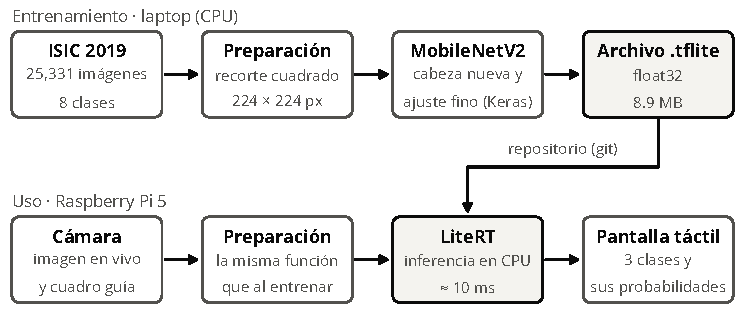
\includegraphics[width=\textwidth]{figuras/fig_sistema.pdf}
\caption{Arquitectura de Computer Vision DermaCheck. Arriba, las etapas que corren una sola vez en la laptop; abajo, el uso diario en la Raspberry Pi 5. La función de preparación de la imagen es idéntica en ambos lados, de modo que la red recibe en la placa exactamente el mismo tipo de entrada con el que aprendió.}\label{fig1}
\end{figure}

\subsection{Entrenamiento}\label{subsec2}

El entrenamiento completo duró 44.6 minutos en el CPU de una laptop con procesador Apple M4, sin aceleración gráfica. La primera fase, en la que solo aprende la capa final, avanzó despacio: tras seis épocas el recall promedio de validación apenas llegó a 0.441 (Fig.~\ref{fig2}). El salto vino al descongelar las últimas 40 capas de MobileNetV2. Tras un tropiezo en la primera época de esa fase, la curva subió con rapidez, y cuando el paso de aprendizaje se redujo a la mitad, en la época 17, el recall ganó más de nueve centésimas de golpe. El máximo, 0.670, apareció en la época 19, y ese es el modelo que conservamos.

\begin{figure}[t]
\centering
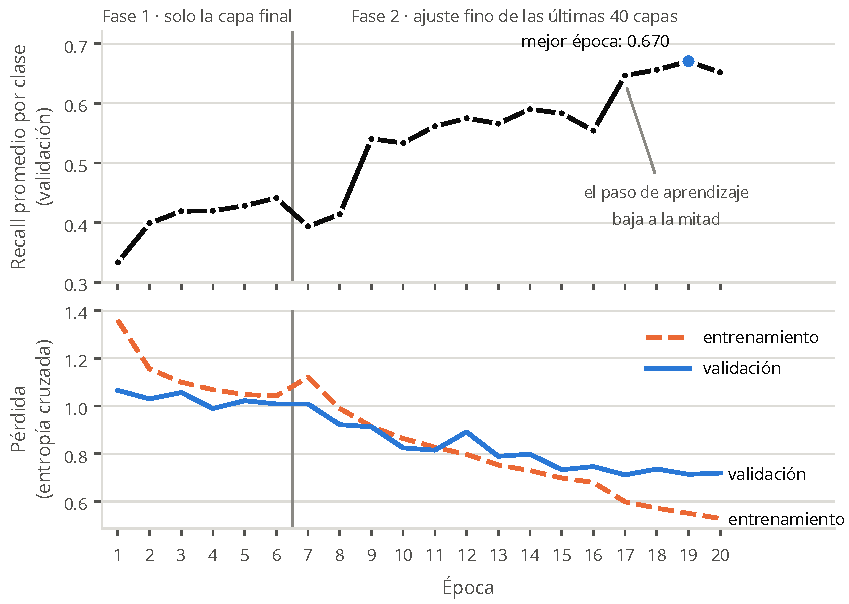
\includegraphics[width=\textwidth]{figuras/fig_entrenamiento.pdf}
\caption{Evolución del entrenamiento. Arriba, el recall promedio por clase en el conjunto de validación, que es la métrica que decidió qué pesos conservar; abajo, la pérdida en entrenamiento y en validación. La línea vertical separa la fase en la que solo aprende la capa final de la fase de ajuste fino.}\label{fig2}
\end{figure}

La pérdida de validación se estabilizó cerca de 0.71 mientras la de entrenamiento seguía bajando hasta 0.53. Esa brecha creciente indica que la red empezaba a memorizar detalles del conjunto de entrenamiento, y es otra razón para no alargar la segunda fase sin más datos o más aumento de imágenes.

\subsection{Desempeño en el conjunto de prueba}\label{subsec3}

Evaluamos el modelo una sola vez sobre 5,067 imágenes reservadas desde el inicio, que no intervinieron ni en el ajuste de los pesos ni en la elección de la mejor época. La exactitud global fue de 0.725 (3,672 aciertos) y el recall promedio por clase, de 0.632, algo por debajo del 0.670 de validación. La Tabla~\ref{tab1} desglosa el resultado por categoría.

\begin{table}[h]
\caption{Desempeño por clase en el conjunto de prueba (modelo float32). El recall indica qué fracción de las lesiones de cada clase reconoció el modelo; la precisión, qué fracción de sus predicciones de esa clase fue correcta.}\label{tab1}%
\begin{tabular}{@{}lllll@{}}
\toprule
Clase & Precisión & Recall & F1 & Imágenes\\
\midrule
AK, queratosis actínica      & 0.425 & 0.451 & 0.437 & 182 \\
BCC, carcinoma basocelular   & 0.665 & 0.792 & 0.723 & 606 \\
BKL, queratosis benigna      & 0.483 & 0.615 & 0.541 & 507 \\
DF, dermatofibroma           & 0.234 & 0.595 & 0.336 & 42 \\
MEL, melanoma                & 0.761 & 0.471 & 0.582 & 949 \\
NV, nevo melanocítico        & 0.850 & 0.855 & 0.852 & 2,606 \\
SCC, carcinoma escamoso      & 0.422 & 0.419 & 0.421 & 117 \\
VASC, lesión vascular        & 0.667 & 0.862 & 0.752 & 58 \\
\midrule
Promedio por clase           & 0.563 & 0.632 & 0.580 & 5,067 \\
Promedio ponderado           & 0.742 & 0.725 & 0.725 & 5,067 \\
\botrule
\end{tabular}
\footnotetext{La exactitud global es 0.725. Los promedios ponderados usan como peso el número de imágenes de cada clase, por lo que reflejan sobre todo el comportamiento con los nevos, que son la mitad del conjunto.}
\end{table}

Las cifras más altas corresponden a los nevos (0.855) y a las lesiones vasculares (0.862), cuyo aspecto rojizo y bien delimitado las vuelve fáciles de separar. En el otro extremo quedan el carcinoma escamoso (0.419), la queratosis actínica (0.451) y el melanoma (0.471). La matriz de confusión de la Fig.~\ref{fig3} explica buena parte de esos tropiezos: de los 949 melanomas, 298 (31.4\,\%) fueron tomados por nevos y 111 (11.7\,\%) por queratosis benignas, y un tercio de los carcinomas escamosos se confundió con carcinomas basocelulares. El dermatofibroma muestra la combinación contraria, buen recall con precisión muy baja (0.234): el modelo lo propone con frecuencia para lesiones que no lo son, efecto esperable del peso alto que recibió esa clase tan escasa.

\begin{figure}[t]
\centering
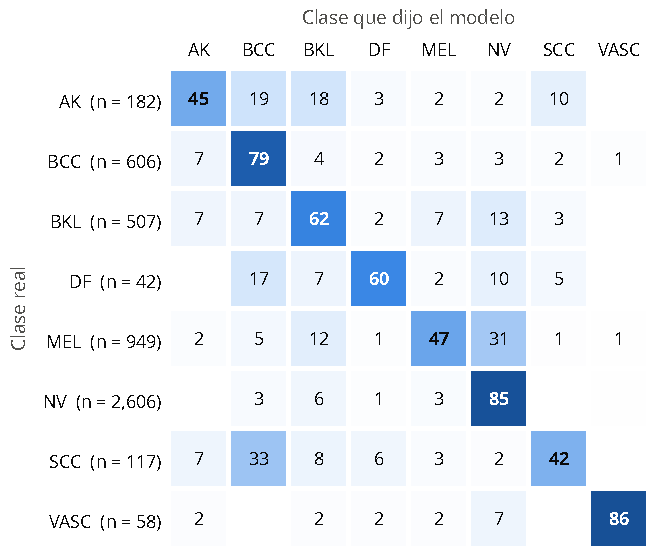
\includegraphics[width=0.78\textwidth]{figuras/fig_confusion.pdf}
\caption{Matriz de confusión en el conjunto de prueba, normalizada por filas: cada celda indica qué porcentaje de las lesiones de una clase real recibió cada etiqueta. La diagonal corresponde a los aciertos y $n$ es el número de imágenes de cada clase. Se omiten los valores menores a 0.5\,\%.}\label{fig3}
\end{figure}

Si agrupamos las tres clases malignas (melanoma, carcinoma basocelular y carcinoma escamoso) contra el resto, el modelo identifica como maligna alguna de esas tres en 1,102 de 1,672 lesiones malignas, una sensibilidad de 0.659, y descarta correctamente 3,072 de 3,395 lesiones no malignas, una especificidad de 0.905.

\subsection{Modelo completo y modelo ligero}\label{subsec4}

Exportamos dos versiones del modelo. La primera conserva los pesos en punto flotante de 32 bits; la segunda los cuantiza a enteros de 8 bits, lo que reduce el archivo de 8.9 a 2.5\,MB. La Tabla~\ref{tab2} compara ambas. La versión float32 reprodujo las probabilidades del modelo original con una diferencia máxima de $9.2\times10^{-6}$ en las 5,067 imágenes, así que para fines prácticos es el mismo modelo. La ligera, en cambio, eligió la misma clase que el original en el 94.5\,\% de las imágenes y perdió entre uno y 1.4 puntos de recall promedio.

\begin{table}[h]
\caption{Comparación de las dos versiones exportadas. Las métricas son sobre las 5,067 imágenes de prueba; los tiempos de la Raspberry Pi 5 se midieron clasificando una imagen a la vez.}\label{tab2}%
\begin{tabular*}{\textwidth}{@{\extracolsep\fill}lcc}
\toprule
 & float32 & Ligero (int8) \\
\midrule
Tamaño del archivo & 8.9 MB & 2.5 MB \\
Exactitud & 0.725 & 0.721--0.722\footnotemark[1] \\
Recall promedio por clase & 0.632 & 0.619--0.623\footnotemark[1] \\
Misma clase que el modelo de Keras & 100\,\% & 94.5\,\% \\
Tiempo por imagen en la Pi, 1 hilo & 21.7 ms & 19.0 ms \\
Tiempo por imagen en la Pi, 4 hilos & 9.7 ms & 11.5 ms \\
\botrule
\end{tabular*}
\footnotetext{Con 2 hilos, la versión float32 tardó 12.7\,ms por imagen en la Pi.}
\footnotetext[1]{El primer valor se obtuvo en la laptop que hizo la exportación y el segundo en la Raspberry Pi; la diferencia se discute en el texto.}
\end{table}

Un detalle nos sorprendió. Con la versión float32, las probabilidades de la Pi y las de la laptop difirieron en menos de tres millonésimas. Con la ligera no: la laptop que hizo la exportación obtuvo un recall promedio de 0.619 y la Pi, de 0.623, con diferencias de hasta 0.015 en las probabilidades de las imágenes de muestra. Todo apunta a las rutinas de cálculo entero que el intérprete elige para cada procesador: la misma laptop, con una versión anterior del intérprete, reproduce exactamente los resultados de la Pi. Como la versión ligera además fue más lenta con cuatro hilos, la aplicación usa la float32.

\subsection{Funcionamiento en la Raspberry Pi 5}\label{subsec5}

Clasificamos en la propia Pi las 5,067 imágenes de prueba, una por una, como lo hace la aplicación. Con la versión float32, la clase elegida coincidió con la de la laptop en todos los casos. Con los cuatro núcleos, cada imagen tardó 9.7\,ms, lo que daría para clasificar unas cien imágenes por segundo; en la práctica la aplicación solo clasifica cuando el usuario toca el botón, así que el tiempo de respuesta lo domina la interfaz y no la red.

La parte complicada resultó ser la energía. Durante las primeras pruebas la placa se apagó dos veces sin aviso, así que repetimos la clasificación completa registrando cada dos segundos la temperatura, el voltaje de la línea de 5\,V y las alertas del firmware. La Tabla~\ref{tab3} resume lo que encontramos.

\begin{table}[h]
\caption{Pruebas de carga en la Raspberry Pi 5 sin ventilador, clasificando continuamente el conjunto de prueba. Ambas fuentes negociaron 3\,A a 5\,V; la fuente oficial de la placa entrega 5\,A.}\label{tab3}%
\begin{tabular*}{\textwidth}{@{\extracolsep\fill}llccl}
\toprule
Alimentación & Hilos & Temp. máx. & 5\,V mín. & Resultado \\
\midrule
USB-C de laptop & 1 & 67.5\,\textdegree C & 4.81\,V & Estable \\
USB-C de laptop & 2 & 84.5\,\textdegree C & 4.78\,V & Estable, con freno térmico \\
USB-C de laptop & 4 & --\footnotemark[1] & 4.70\,V & Se apagó a los 2\,s \\
Cargador de 65\,W & 4 & 87.3\,\textdegree C & 4.76\,V & Estable, 7 avisos de voltaje \\
\botrule
\end{tabular*}
\footnotetext[1]{La placa se apagó antes de que la temperatura subiera; la última lectura fue de 75.2\,\textdegree C.}
\end{table}

Conectada al puerto USB-C de una laptop, la Pi soportó uno y dos núcleos, pero al arrancar los cuatro el voltaje cayó a 4.70\,V, el sistema registró una alerta de bajo voltaje y dos segundos después la placa quedó apagada. Con un cargador de pared de 65\,W, que también negocia solo 3\,A a 5\,V, resistió unos cuatro minutos de carga casi continua, aunque con siete alertas breves de bajo voltaje. La temperatura fue el segundo límite: sin disipador, la placa llegó a 87.3\,\textdegree C, redujo su frecuencia hasta 1.5\,GHz durante cerca de 48 segundos y el tiempo por imagen subió de 9.7 a 11.9\,ms. Sumando los rieles internos que reporta el controlador de energía, la placa consumió unos 2\,W en reposo y alrededor de 7\,W con los cuatro núcleos ocupados; la documentación del fabricante recomienda para este modelo una fuente de 5\,A \cite{rpi5_power,rpi_27w}.

\subsection{La aplicación}\label{subsec6}

La Fig.~\ref{fig4} muestra las dos pantallas de la aplicación en el tamaño de la pantalla táctil de siete pulgadas que usaremos (1024\,$\times$\,600 píxeles). En la primera, la imagen en vivo aparece oscurecida salvo un cuadro central con una retícula; ese cuadro es exactamente la región que se clasifica. Al tocar «Tomar», la segunda pantalla presenta la clase más probable con su porcentaje, una escala de 0 a 100 con la posición de las tres primeras clases y un aviso permanente de que el resultado no es un diagnóstico. Si alguna de las clases de riesgo (melanoma, carcinomas o queratosis actínica) alcanza 25\,\% entre las tres primeras, aparece en color ámbar la sugerencia de acudir a un dermatólogo; si la clase principal no llega a 50\,\%, la aplicación advierte que el resultado es poco seguro.

\begin{figure}[t]
\centering
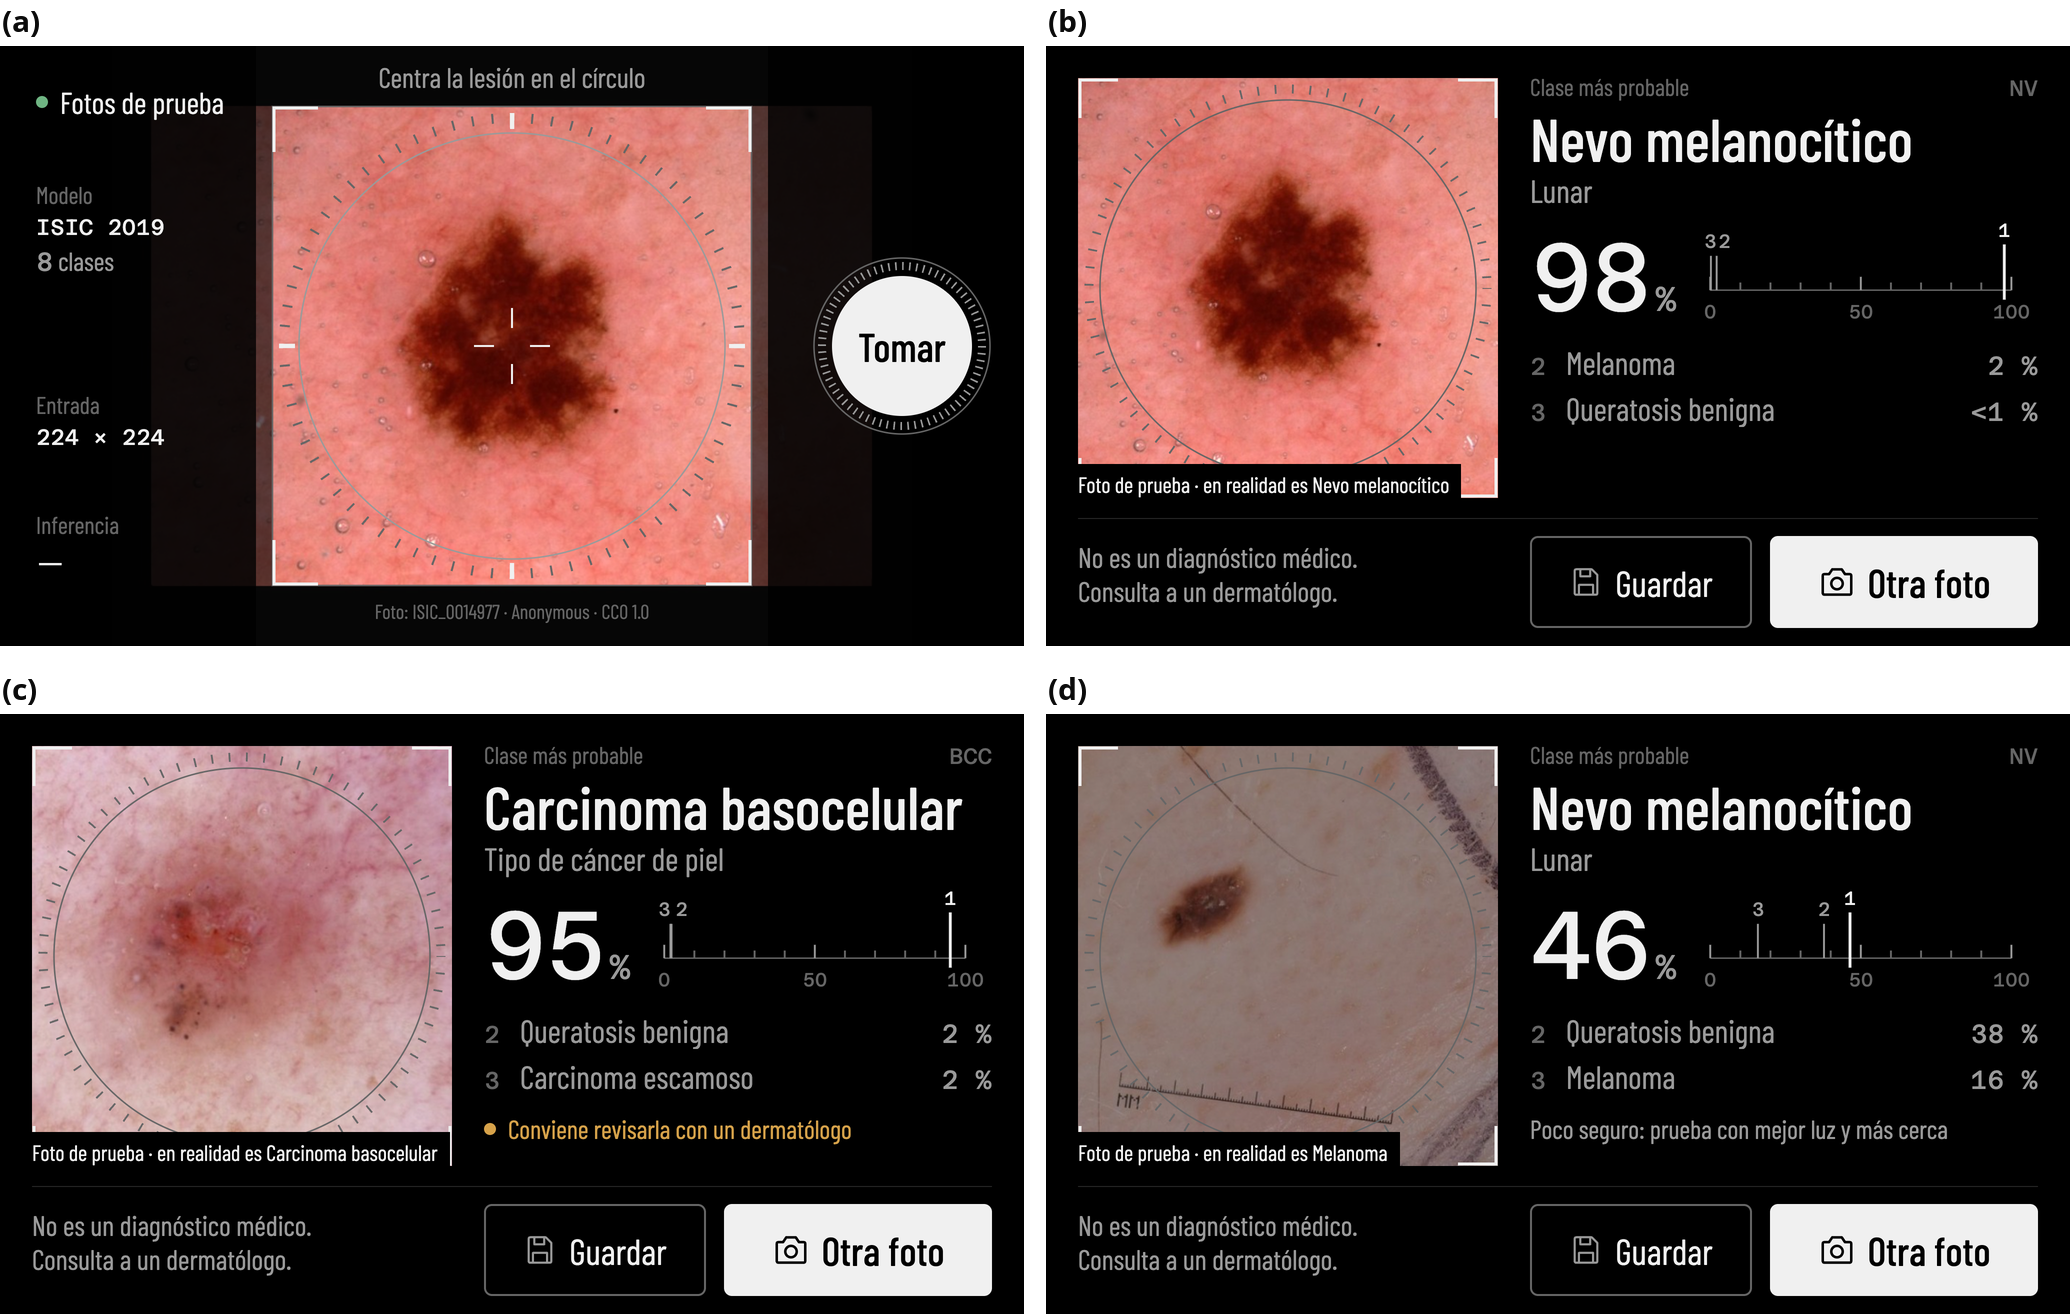
\includegraphics[width=\textwidth]{figuras/fig_app.png}
\caption{Capturas de la aplicación con imágenes de prueba de ISIC. (a) Pantalla de cámara con el cuadro guía, que coincide con la región que se clasifica. (b) Nevo reconocido con 98\,\%. (c) Carcinoma basocelular reconocido con 95\,\%; el aviso ámbar sugiere consultar a un dermatólogo. (d) Un melanoma que el modelo confunde con un nevo, con solo 46\,\% y la advertencia de resultado poco seguro.}\label{fig4}
\end{figure}

Para demostrar el sistema sin cámara, la aplicación incluye un modo de prueba que recorre 62 fotografías con licencia abierta: 40 dermatoscópicas del propio ISIC, cinco por clase y elegidas al azar, y 22 clínicas de Wikimedia Commons, tomadas con cámaras comunes. El modelo acertó la clase de 24 de las 40 imágenes dermatoscópicas y solo de 7 de las 22 clínicas. Son muestras pequeñas, pero la caída coincide con lo que esperábamos de un modelo que aprendió únicamente con imágenes de dermatoscopio.

\section{Métodos}\label{sec11}

\subsection{Conjunto de datos}\label{subsec7}

Usamos el conjunto de entrenamiento del reto ISIC 2019, que reúne 25,331 imágenes dermatoscópicas de ocho categorías diagnósticas \cite{isic2019,isic2019datos}. Las imágenes provienen de tres colecciones: HAM10000, con 10,015 imágenes \cite{tschandl2018}; BCN20000, del Hospital Clínic de Barcelona \cite{hernandezperez2024}; y las del reto ISIC 2017 \cite{codella2018}. Trabajamos con una copia publicada en Hugging Face que ya divide las imágenes en 20,264 para entrenar y 5,067 para probar \cite{hf_isic2019}; ambas partes suman exactamente las 25,331 imágenes del conjunto de entrenamiento oficial, de modo que nuestra prueba es una porción reservada de ese conjunto y no la prueba oficial del reto. De las 20,264 imágenes separamos de forma estratificada el 10\,\% para validación (2,027) y dejamos 18,237 para ajustar los pesos. La Tabla~\ref{tab4} muestra el reparto, y la Fig.~\ref{fig5}, un ejemplo de cada clase.

\begin{table}[h]
\caption{Número de imágenes por clase en cada partición.}\label{tab4}%
\begin{tabular*}{\textwidth}{@{\extracolsep\fill}lrrrr}
\toprule
Clase & Entrenamiento & Validación & Prueba & Total \\
\midrule
AK, queratosis actínica    & 616   & 69    & 182   & 867 \\
BCC, carcinoma basocelular & 2,445 & 272   & 606   & 3,323 \\
BKL, queratosis benigna    & 1,905 & 212   & 507   & 2,624 \\
DF, dermatofibroma         & 177   & 20    & 42    & 239 \\
MEL, melanoma              & 3,216 & 357   & 949   & 4,522 \\
NV, nevo melanocítico      & 9,242 & 1,027 & 2,606 & 12,875 \\
SCC, carcinoma escamoso    & 460   & 51    & 117   & 628 \\
VASC, lesión vascular      & 176   & 19    & 58    & 253 \\
\midrule
Total                      & 18,237 & 2,027 & 5,067 & 25,331 \\
\botrule
\end{tabular*}
\footnotetext{La categoría BKL agrupa lentigo solar, queratosis seborreica y queratosis liquenoide. El desbalance es extremo: en la partición de entrenamiento hay 52 nevos por cada dermatofibroma.}
\end{table}

\begin{figure}[t]
\centering
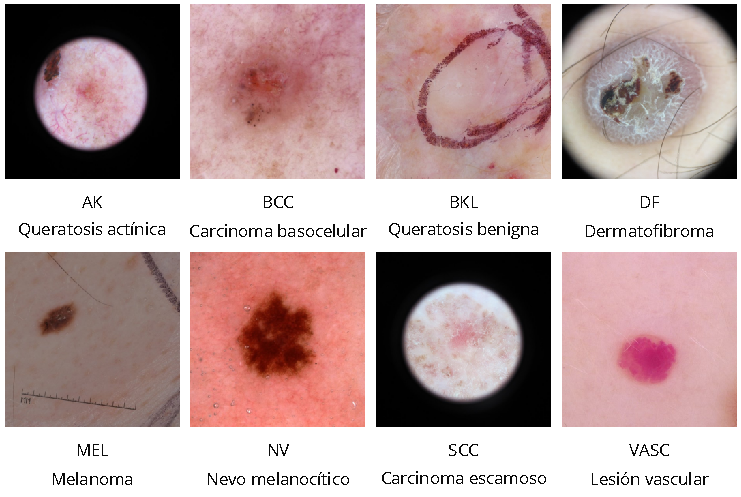
\includegraphics[width=\textwidth]{figuras/fig_clases.pdf}
\caption{Una imagen de prueba de cada clase, con el mismo recorte cuadrado que recibe la red. Los créditos y licencias de cada imagen están en el Apéndice~\ref{secA1}.}\label{fig5}
\end{figure}

\subsection{Preparación de las imágenes}\label{subsec8}

Cada imagen pasa por la misma función antes de entrar a la red: se corrige su orientación según los metadatos EXIF, se convierte a RGB, se recorta el cuadrado central más grande posible y se reduce a 224\,$\times$\,224 píxeles con interpolación bilineal. La Raspberry Pi usa una copia de esa función, y una prueba automática verifica que ambas producen exactamente los mismos píxeles. La red recibe valores entre 0 y 255; la conversión al intervalo que espera MobileNetV2 ocurre dentro del propio modelo,
\begin{equation}
\tilde{x} = \frac{x}{127.5} - 1,\label{eq1}
\end{equation}
de modo que el programa de la placa no tiene que repetir ese paso. Durante el entrenamiento añadimos variaciones aleatorias a cada imagen: giros horizontales y verticales, rotaciones de hasta media vuelta en cualquier sentido, cambios de escala de hasta 15\,\% y variaciones de brillo y contraste de la misma magnitud. Estas transformaciones solo existen al entrenar y no forman parte del modelo exportado.

\subsection{Arquitectura y entrenamiento}\label{subsec9}

MobileNetV2 se construye con bloques residuales invertidos: cada bloque expande una representación compacta, la filtra con convoluciones separables en profundidad y la vuelve a comprimir con una proyección lineal \cite{sandler2018,howard2017}. Cargamos la red sin su clasificador original, con los pesos aprendidos en ImageNet \cite{deng2009}, y le añadimos un promedio global, una capa de \textit{dropout} con tasa 0.3 y una capa densa de ocho salidas con activación softmax. El modelo completo tiene 2,268,232 parámetros. Reutilizar los pesos de ImageNet aprovecha que las primeras capas de una red entrenada con imágenes naturales aprenden rasgos generales, como bordes y manchas de color, que sirven para otras tareas \cite{yosinski2014}.

El entrenamiento siguió dos fases con el optimizador Adam \cite{kingma2015} y lotes de 64 imágenes. En la primera, la red base quedó congelada y solo aprendieron los 10,248 parámetros de la capa final, con un paso de aprendizaje de $10^{-3}$ durante seis épocas. En la segunda descongelamos las últimas 40 capas de MobileNetV2, salvo las de normalización por lotes \cite{ioffe2015}, que se mantuvieron fijas para conservar las estadísticas aprendidas en ImageNet; así quedaron 1,673,608 parámetros entrenables, ajustados con un paso de $10^{-4}$ durante un máximo de 14 épocas. Usamos TensorFlow 2.21 y Keras 3.15 \cite{abadi2016,keras}.

Para compensar el desbalance \cite{he2009}, cada imagen de la clase $c$ contribuye a la pérdida con un peso
\begin{equation}
w_c = \left(\frac{N}{K\,n_c}\right)^{1/2},\label{eq2}
\end{equation}
donde $N$ es el número de imágenes de entrenamiento, $K=8$ el número de clases y $n_c$ las imágenes de la clase $c$. La raíz cuadrada suaviza el efecto: el peso va de 0.50 para los nevos a 3.60 para las lesiones vasculares, en lugar del intervalo de 0.25 a 12.95 que daría la proporción inversa directa. La función que se minimiza es la entropía cruzada ponderada sobre cada lote de $B$ imágenes,
\begin{equation}
\mathcal{L} = -\frac{1}{B}\sum_{i=1}^{B} w_{y_i}\,\log p_{i,y_i},\label{eq3}
\end{equation}
con $y_i$ la clase verdadera de la imagen $i$ y $p_{i,y_i}$ la probabilidad que el modelo le asigna. La Tabla~\ref{tab5} reúne los hiperparámetros.

\begin{table}[h]
\caption{Hiperparámetros del entrenamiento.}\label{tab5}%
\begin{tabular}{@{}lll@{}}
\toprule
Parámetro & Fase 1 & Fase 2 \\
\midrule
Capas entrenables & solo la capa final & últimas 40 de la base y la capa final \\
Paso de aprendizaje inicial & $10^{-3}$ & $10^{-4}$ \\
Épocas máximas & 6 & 14 \\
Parámetros entrenables & 10,248 & 1,673,608 \\
Tamaño de lote & \multicolumn{2}{l}{64} \\
Optimizador & \multicolumn{2}{l}{Adam} \\
\textit{Dropout} & \multicolumn{2}{l}{0.3} \\
Parada temprana & \multicolumn{2}{l}{4 épocas sin mejora del recall promedio} \\
Reducción del paso & \multicolumn{2}{l}{a la mitad tras 2 épocas sin mejora} \\
\botrule
\end{tabular}
\end{table}

\subsection{Selección del modelo y métricas}\label{subsec10}

La exactitud global engaña cuando la mitad de las imágenes son nevos, porque un modelo que dijera «nevo» siempre ya acertaría la mitad de las veces. Por eso elegimos los pesos con el recall promedio por clase en validación,
\begin{equation}
\bar{R} = \frac{1}{K}\sum_{c=1}^{K}\frac{\mathrm{VP}_c}{\mathrm{VP}_c+\mathrm{FN}_c},\label{eq4}
\end{equation}
donde $\mathrm{VP}_c$ son las imágenes de la clase $c$ clasificadas correctamente y $\mathrm{FN}_c$ las que recibieron otra etiqueta. Al terminar cada época calculamos $\bar{R}$; si mejoraba, guardábamos los pesos. Esa misma métrica controló la parada temprana y la reducción del paso de aprendizaje. En la prueba reportamos además la precisión, $\mathrm{VP}_c/(\mathrm{VP}_c+\mathrm{FP}_c)$, y la puntuación F1, que es la media armónica de precisión y recall.

\subsection{Exportación a TensorFlow Lite}\label{subsec11}

El modelo se convirtió al formato de TensorFlow Lite, que Google renombró LiteRT en 2024 \cite{litert,litert_rename}. La versión ligera usa cuantización de rango dinámico: los pesos se guardan como enteros de 8 bits y se traducen a reales mediante la relación afín
\begin{equation}
r = S\,(q - Z),\label{eq5}
\end{equation}
en la que $q$ es el entero almacenado, $S$ una escala y $Z$ el entero que representa al cero \cite{jacob2018}. Durante la inferencia, el intérprete también cuantiza al vuelo las activaciones, y ese paso explica que el resultado varíe ligeramente entre procesadores. Junto con cada modelo exportamos 16 imágenes de prueba con las probabilidades esperadas; al instalar el modelo, la Pi las clasifica y compara sus resultados con los de la laptop, con una tolerancia de $10^{-3}$ para la versión float32 y de 0.05 para la ligera.

\subsection{Hardware y aplicación}\label{subsec12}

El dispositivo es una Raspberry Pi 5 con 8\,GB de memoria, cuyo procesador Broadcom BCM2712 tiene cuatro núcleos Arm Cortex-A76 a 2.4\,GHz \cite{rpi5}, con Raspberry Pi OS de 64 bits, Python 3.13 y el intérprete \texttt{ai-edge-litert} \cite{ai_edge_litert}. La pantalla es táctil, de siete pulgadas y 1024\,$\times$\,600 píxeles, conectada por HDMI. La aplicación consta de un pequeño servidor en Python que lee la cámara y ejecuta el modelo, y de una página que Chromium muestra a pantalla completa; acepta el módulo de cámara de la Raspberry Pi, una cámara web USB o, sin cámara, las fotografías del modo de prueba. Las imágenes solo se guardan si el usuario lo pide. El Algoritmo~\ref{algo1} describe lo que ocurre al tocar «Tomar».

\begin{algorithm}
\caption{Clasificación al tocar «Tomar»}\label{algo1}
\begin{algorithmic}[1]
\Require cuadro más reciente de la cámara $I$ de $w\times h$ píxeles; modelo $M$; fracción del cuadro guía $g=0.8$
\Ensure las tres clases más probables y los avisos que se muestran
\State $s \gets \operatorname{round}(g\cdot\min(w,h))$
\State $C \gets$ cuadrado de lado $s$ centrado en $I$\Comment{la región del cuadro guía}
\State $x \gets$ $C$ reducido a $224\times224$ píxeles con interpolación bilineal
\State $p \gets M(x)$\Comment{ocho probabilidades que suman 1}
\State $T \gets$ las tres clases con mayor $p$
\If{alguna clase de $T$ es MEL, BCC, SCC o AK y su probabilidad es al menos 0.25}\label{algln2}
    \State mostrar el aviso ámbar «Conviene revisarla con un dermatólogo»
\EndIf
\If{$\max p < 0.5$}
    \State mostrar «Poco seguro: prueba con mejor luz y más cerca»
\EndIf
\State \Return $T$ con sus probabilidades
\end{algorithmic}
\end{algorithm}

Para medir el rendimiento en la placa clasificamos las 5,067 imágenes de prueba con uno, dos y cuatro hilos, igual que en la aplicación. Durante esas corridas, un proceso aparte registró cada dos segundos la temperatura del procesador, las alertas de reducción de frecuencia y de bajo voltaje del firmware y el voltaje de la línea de 5\,V que mide el controlador de energía, y guardó los mensajes del sistema en la tarjeta de memoria para conservarlos aunque la placa se apagara.

\textbf{Declaración ética.} El estudio no involucró personas ni muestras humanas. Todas las imágenes provienen de colecciones públicas y anonimizadas, con licencias que permiten su uso académico, y se citan con su crédito correspondiente.

\section{Discusión}\label{sec12}

El resultado más incómodo es también el más importante: el modelo reconoce menos de la mitad de los melanomas. La mayoría de sus errores con esa clase van hacia los nevos, el desliz con peores consecuencias posibles, porque tranquiliza a quien debería consultar. La precisión del melanoma es razonable (0.761), es decir, cuando el modelo dice «melanoma» suele acertar; lo que flaquea es su disposición a decirlo. Parte de la explicación está en los pesos de la Ecuación~\eqref{eq2}: con la raíz cuadrada, el melanoma recibió un peso de 0.84, menor que el de clases mucho más raras, y el modelo terminó inclinado a no proponerlo. Un ajuste del umbral de decisión, o un peso específico para el melanoma, podría intercambiar parte de la precisión por sensibilidad, que en este contexto vale más.

Comparar nuestras cifras con las de la literatura exige cautela. Los trabajos de Esteva y de Haenssle evaluaron tareas binarias, con otros conjuntos y redes más grandes \cite{esteva2017,haenssle2018}, mientras que aquí la red elige entre ocho clases muy desbalanceadas y cabe en un archivo de 9\,MB. Además, la partición entre entrenamiento y prueba no separa por lesión: HAM10000 incluye varias imágenes de una misma lesión, y si algunas quedaron de ambos lados, las cifras resultan algo optimistas. Aun con esas reservas, que una red de 2.3 millones de parámetros entrenada en 45 minutos sin tarjeta gráfica distinga nevos, carcinomas basocelulares y lesiones vasculares con recall superior a 0.79 dice bastante de lo accesible que se ha vuelto esta tecnología.

La experiencia con la Raspberry Pi dejó una lección práctica. La inferencia fue lo más sencillo, pues cada imagen tarda menos de 10\,ms; lo que puso en riesgo el funcionamiento fueron la fuente y el calor. Una placa alimentada desde una laptop se apaga en cuanto se le exige todo el procesador, y una sin disipador se frena por temperatura en uno o dos minutos. Para una demostración confiable bastan la fuente oficial de 27\,W y un disipador activo, o bien limitar el modelo a dos hilos, que con 12.7\,ms por imagen sigue siendo de sobra rápido.

La limitación de fondo es el tipo de imagen. El modelo aprendió con fotografías de dermatoscopio, tomadas pegadas a la piel y con luz controlada, y su acierto bajó de 24 de 40 imágenes dermatoscópicas a 7 de 22 fotos clínicas. Con una cámara común sucederá algo parecido, y lo mismo con tonos de piel poco representados en ISIC, una carencia ya documentada en otros sistemas \cite{daneshjou2022}. El paso natural sería acoplar a la cámara un lente dermatoscópico económico y reentrenar con imágenes más diversas. También conviene añadir una forma de reconocer cuando la imagen no muestra una lesión, porque hoy el modelo siempre elige una de las ocho clases, incluso frente a una foto de una mano o de una taza.

\section{Conclusión}\label{sec13}

Computer Vision DermaCheck demuestra que un clasificador de lesiones cutáneas puede entrenarse en una laptop y funcionar en una placa de bajo costo sin perder exactitud en el traslado: la Raspberry Pi reprodujo, imagen por imagen, las predicciones de la computadora donde se entrenó. Su desempeño, en cambio, todavía no alcanza para confiar en él frente a un melanoma, y por eso la aplicación insiste en que no diagnostica. El valor del prototipo está en otra parte, en volver tangible para un salón de clases cómo aprende una red neuronal, dónde se equivoca y por qué, y en dejar medido qué hace falta para llevarla de una computadora a un dispositivo que cabe en la mano.

\backmatter

\bmhead{Información suplementaria}

El código del proyecto, los cuadernos de entrenamiento y evaluación, el modelo exportado, los registros de las pruebas en la Raspberry Pi y los créditos de las 62 imágenes del modo de prueba están en el repositorio del proyecto, disponible a solicitud de los autores.

\bmhead{Agradecimientos}

Agradecemos a la International Skin Imaging Collaboration y a las instituciones que donaron las imágenes de ISIC 2019, a quien publicó en Hugging Face la copia del conjunto con la que trabajamos y a los fotógrafos de Wikimedia Commons que compartieron sus imágenes con licencia abierta.

\section*{Declaraciones}

\begin{itemize}
\item \textbf{Financiamiento:} el proyecto no recibió financiamiento; el equipo cubrió el costo del hardware.
\item \textbf{Conflicto de intereses:} los autores declaran no tener conflictos de intereses.
\item \textbf{Aprobación ética y consentimiento para participar:} no aplica; el estudio usó solo imágenes públicas y anonimizadas.
\item \textbf{Consentimiento para publicación:} no aplica.
\item \textbf{Disponibilidad de datos:} el conjunto ISIC 2019 está disponible en el sitio del reto \cite{isic2019datos} y la copia utilizada, en Hugging Face \cite{hf_isic2019}. Las métricas y registros de este trabajo están en el repositorio del proyecto.
\item \textbf{Disponibilidad de materiales:} no aplica.
\item \textbf{Disponibilidad del código:} disponible a solicitud de los autores.
\item \textbf{Contribución de los autores:} todos los autores participaron en la concepción del proyecto, la preparación de los datos, el entrenamiento y la evaluación del modelo, el montaje del prototipo y la redacción del manuscrito, y aprobaron la versión final.
\end{itemize}

\begin{appendices}

\section{Créditos de las imágenes}\label{secA1}

Las imágenes de la Fig.~\ref{fig5} y de la Fig.~\ref{fig4} pertenecen al archivo de ISIC. La Tabla~\ref{tabA1} indica el identificador, el autor y la licencia de cada una, según el propio archivo.

\begin{table}[h]
\caption{Créditos de las imágenes de ISIC usadas en las figuras.}\label{tabA1}%
\begin{tabular}{@{}llll@{}}
\toprule
Identificador & Clase & Autor & Licencia \\
\midrule
ISIC\_0062738 & AK   & Hospital Clínic de Barcelona & CC BY-NC 4.0 \\
ISIC\_0029546 & BCC  & MILK study team              & CC BY-NC 4.0 \\
ISIC\_0012323 & BKL  & Anónimo                      & CC0 1.0 \\
ISIC\_0071844 & DF   & Hospital Clínic de Barcelona & CC BY-NC 4.0 \\
ISIC\_0012425 & MEL  & Anónimo                      & CC0 1.0 \\
ISIC\_0014977 & NV   & Anónimo                      & CC0 1.0 \\
ISIC\_0071727 & SCC  & Hospital Clínic de Barcelona & CC BY-NC 4.0 \\
ISIC\_0029439 & VASC & MILK study team              & CC BY-NC 4.0 \\
\botrule
\end{tabular}
\footnotetext{La Fig.~\ref{fig4} usa ISIC\_0014977, ISIC\_0029546 e ISIC\_0012425.}
\end{table}

\end{appendices}

%%===========================================================================================%%
%% If you are submitting to one of the Nature Portfolio journals, using the eJP submission   %%
%% system, please include the references within the manuscript file itself. You may do this  %%
%% by copying the reference list from your .bbl file, paste it into the main manuscript .tex %%
%% file, and delete the associated \verb+\bibliography+ commands.                            %%
%%===========================================================================================%%

\bibliography{sn-bibliography}% common bib file
%% if required, the content of .bbl file can be included here once bbl is generated
%%\input sn-article.bbl

\end{document}
